\section{Anforderungsanalyse}


\subsection{VJing}

Die Pr\"asentation von visuellem Material setzt gewisse Technik vorraus, welches verschiedene Medienformate unterst\"utzt,
andere nur unter Umst\"anden und manches vielleicht gar nicht. Beispielsweise unterst\"utzt ein Videorecorder keine digitalen
Videodateien. M\"ochte man die Performance mithilfe von Videoclips realisieren und braucht Funktionen wie Zeitraffer oder
automatisches Vorw\"arts-R\"uckw\"arts-Abspielen ist eine Software gesucht die das kann. Legt man viele Videos \"ubereinander 
setzt das gewisse Rechenressourcen vorraus, mit denen das Resultat dargestellt wird.

Vor allem auf der Softwareseite sind viele Abh\"angigkeiten zu beachten. Da bei dem VRC-Konzept das Abspielen von Videoclips
nicht verloren gehen soll, die Darstellung und Animation von 3D-Inhalten zu Musik prim\"ares Ziel sind, stellt sich die Frage
mit welche Libraries in Frage kommen.

Der Bedienbarkeit kommt auch ein eigenes Feld zu. Viele VJs benutzen MIDI Controller, um die Darstellung zu steuern, da 
Potentiometer gef\"uhlvolles Einstellen von Parametern erm\"oglicht. Gleichzeitig muss ein VJ auf drastische \"Anderungen 
an der Darstellung vorbereitet sein.

\subsubsection{Hardware und Software}

Die Hardware sollte mobil sein. Ein Videoprojektor und ein Laptop sind die Grundlage f\"ur das Performen. F\"ur die 
Soundanalyse kann man direkt das Signal von einem Verst\"arker abgreifen oder \"uber ein Mikrofon aufnehmen. Gleichzeitiges 
Abspielen von mehreren Visuals auf einmal sollte m\"oglich sein. Das Anordnen der Visuals in einem dreidimensionalen
Raum erfordert Software, die das kann und auf Hardwareseite ist 3D-Beschleunigung n\"otig. 
\\
Ein Laptop, der mehrere Videoclips und 3D-Modelle auf einmal berechnet und dazu den Sound analysiert und mit der Szenerie
verkn\"upft um Animationen und Visualit\"at zu erzeugen, braucht ein gewisses Mass an Rechenkraft. Da nicht nur die 
Grafikkarte zum Rendern beansprucht wird, sondern vor allem auch die CPU f\"ur das schnelle Analysieren des Sounds und 
Ausf\"uhren von Funktionen zust\"andig ist, darf hier nicht gespaart werden. Je nach dem wie Aufw\"andig die Szenerie
gestaltet ist ergeben sich Mengen von Polygonen, die transformiert werden m\"ussen. Auch hier sollten gen\"ugend 
Leistungsreserven vorhanden sein, weshalb von Integrierten Grafikkarten abzuraten ist, da dedizierte Grafikkarten 
momentan mehr Leistung haben.

Laptops, die f\"ur Computerspiele, technisches Zeichnen, Bilder- und Videoverarbeitung  konstruiert sind 
verf\"ugen meist schon \"uber eine dedizierte Grafikkarte und eine besserer CPU als regul\"arer B\"urorechner.
\\
Hinsichtlich Kosten und Plattformwahl soll m\"oglichst freie Software verwendet werden. Eine leicht erlernbare 
Programmiersprache zur Erstellung von Visuals soll es VJs mit mit geringen Programmierkenntnissen erm\"oglichen Visuals
f\"ur das Pr\"asentationsprogramm zu programmieren. Eine freie Grafikbibliothek wie OpenGL bietet eine Grundlage f\"ur 
Rendering der Szenerie, jedoch stellt das Programmieren von OpenGL eine gro\ss e H\"urde f\"ur VJs mit nicht so tiefen
Programmierkenntnissen dar. Deher muss es die Komplexit\"at von OpenGL vereinfacht werden und Bibliotheken die auf OpenGL
aufsetzen benutzt werden.


\subsubsection{Bedienbarkeit}

F\"ur die Bedienung sollen standard Eingabeger\"ate wie Tastatur und Maus gen\"ugen. Vor allem die Einstellung der Ansicht
und Positionierung der Visuals in einem 3D-Raum muss auf einer Tastatur komfortabel m\"oglich sein - und das 
wom\"oglich stundenlang. \"Uberblendungen und Visualwechsel beinhalten viele Aktionen wie das \"Andern von Transparenzen oder
Farben und muss fl\"ussig machbar sein. Die Ansicht durch eine virtuelle Kamera erfordert eine bewegliche Kamera. Bei 
Rotationen der Kamera ist es wichtig die Orientierung nicht zu verlieren.

Eine Kombination aus Spielsteuerung f\"ur das ansteuern der Visual-Objekte und der Kamera scheint mit einer Tastatur 
realisierbar und sinnvoll. Das Anzeigen und Einstellen von Statusinformationen von Kamera,
Soundanalyse und aktiven Visuals sowie die \"Ubersicht der verf\"ugbaren Visuals erfordert eine geeignete 
Benutzerschnittstelle mit Panelen an denen Parameter abgelesen und ge\"andert werden k\"onnen.

Wichtig ist eine Reservierung von Tasten auf der Tastatur  f\"ur die Steuerung der ins Visual individuell einprogrammierten
Routinen.


\subsection{Visuals}

In dem VJ-Konzept ist der Fokus auf eine liberale Visualgestaltung ausgerichtet. Operationen wie Verschieben, Skalieren, 
Rotieren und transformation zu Musik sollen jedem Visual aufgrund seines Charakters als Objekt in einem 3D-Raum m\"oglich sein. 
Der Sound
soll von Visuals genutzt werden k\"onnen um Effekte auszul\"osen oder zu beeinflussen. Visuals bestehen bspw aus Punkten die zu 
geometrischen Formen verbunden werden k\"onnen. Vorgefertigte 3D-Modelle sollen unterst\"utzt werden. Texturen k\"onnen 
aus Bilddateien, Shaderprogrammen oder Videoclips bestehen. Durch das Programmieren der Visuals hat man 
die M\"oglichkeit eigene Bibliotheken zu benutzen und Algorithmen zur Visualisierung zu implementieren. 
 
\subsubsection{Erstellen}

F\"ur das Erstellen von Visuals ist es wichtig, dass der K\"unstler seine Visualidee verwirklichen kann. G\"angige 
Formate f\"ur Bilddateien und Videos m\"ussen unterst\"utzt werden. Dadurch hat der (VJ)K\"unstler die M\"oglichkeit
verschiedene Tools zu benutzen um Bilder oder Videos zu pr\"aparieren. Im 3D-Raum k\"onnen diese dann als Texturen auf
Fl\"achen dargestellt werden. 

Vor allem soll aber der VJ auch Punkte zu Poligonnetzen verbinden k\"onnen. So k\"onnen 3D-Modelle mit 3D-Grafikprogrammen
wie bspw Blender erstellt und in Visuals verwendet werden. Dadurch ist es auch m\"oglich vorgefertigte 3D-Modelle aus dem
Internet zu benutzen, welche von Anbietern zum Beispiel f\"ur CAD (Computer Aided Design), oder Spiele zum Download bereitgestellt 
werden. Manche Formate bieten die M\"oglichkeit Animationen zu direkt im Model zu definieren. Unabh\"angig von Formaten
m\"ussen die Inhalte auch durch selbstgeschriebene Funktionen animierbar sein. 

Mit eigens definierten Funktionen kann man auf die Skalierung, Farbe, Transparenz oder Positionierung Einfluss nehmen.
Das Soundsignal als wichtiger Bestandteil muss in Funktionen verarbeitbar sein. Durch die Analyse des Soundsignals k\"onnen 
sich Funktionen dynamisch gegenseitig aufrufen und mit der k\"unstlerischen Intention verkn\"upft werden. So kann das 
Visual programmiert werden auf B\"asse vorprogrammierte Effekte auszul\"osen.

Mit der Programmierung der Tasteneingabe kann das Visual gesteuert werden. Die Zustandsa\"nderung auf eine Tasteneingabe
muss bei der Erstellung definiert werden k\"onnen. Auch hierbei sind Funktionen die Grundlage daf\"ur.

primitive, 3d meshes, 
fertige modelle mit blender
videoclips
tastenbelegung


\subsection{Darstellung}

Ein Programm zur Darstellung der Visuals ist n\"otig um alle Visuals mit dem Soundsignal zu versorgen, Eingaben entgegen
nimmt und auf Parameter der Visuals zugreiffen kann. 


Das Programm stellt den 3D-Raum bereit in denen die Visuals geladen werden k\"onnen sowie eine \"Ubersicht \"uber
Parameter, Eingaben und Metainformationen \"uber die Zust\"ande der Visuals. Eine \"Ubersicht \"uber die Positionen
der Visuals und Kameras sowie der Ausrichtung der Kamera hilft dabei Szenen und Kameraeinstellungen zu koordinieren.

Diese Anforderungen k\"onnen in einer GUI untergebracht werden. Eine GUI fasst dabei Eingabeschnittstellen f\"ur die Visuals,
die Kameras und Soundeinstellungen zusammen, an denen die wichtige Daten \"uber den Zustand des Dargestellten abgelesen
werden k\"onnen.

Eine Ansicht durch eine Kamera wird dabei in Vollbildschirmmodus an das Ausgabeger\"at (Videoprojektor) geschickt. Eine 
andere Ansicht in den Raum erm\"oglicht das direkte Interagieren mit Visuals und Kamera. Diese Ansicht soll den
Computerspielcharakter bereitstellten wodurch direkte Manipulation an Rotation und Position m\"oglich ist.

%Dabei m\"ussen verschiedene Tasks ausgef\"uhrt werden.
%programm zur das sound verarbeitet, 
%parameter einstellung
%taskmanager, 
%Eingabe verarbeiten

%\subsubsection{3D Raum und Camera}

%Durch die Ansicht des 3D-Raums durch die virtuelle Kamera wird der 3D-Raum zum Beh\"alter f\"ur Visuals, der betrachtet wird.
%Die Positionierung der Kamera und der Visuals

%container fuer visuals
%beinhaltet cameras zur ansicht
%Camerapositionierung

\subsubsection{Performen}

Die Performance des VJs besteht aus dem Laden und Entfernen von Visuals in dem 3D-Raum. Visuals werden um die
Kamera angeordnet und bilden die Szenerie. Bei \"Anderungen in der Musik wird die Szenerie angepasst oder der
Blickwinkel auf die Szenerie ge\"andert. 

Musik enth\"alt oft H\"ohepunkte und viele k\"unstlerische Stilmittel.
Anhand der akustischen Wahrnehmung des VJs kann an Wendepunten in der Musik in Echtzeit die Performance des VJs
an die Musik anpasst werden. Durch hineinfaden eines anderen Visuals, einem Schnitt oder dem Ausl\"osen eines 
Effekts erh\"alt die Musik ihre visuelle Individualit\"at w\"ahrend des Events.

Dabei soll das Programm Operationen wie Schnitte, Kamerafahrten, Positionierung und Rotationen, Fading oder
\"Anderungen an der Kameraeinstellung schnell auf Visual und Kamera f\"ur den VJ schell ausf\"uhrbar gestalten.
Hauptaugenmerk f\"ur das Performen ist die Usability. Da die Eingabeger\"ate f\"ur den Anfang aus 
Maus und Tastatur bestehen muss ein geeignetes Bedienkonzept erarbeitet werden.

\section{Entwurf}

Beim Entwurf m\"ussen \"Uberlegungen getroffen werden, welche die Auswahl der Software im Vorfeld auf
die in Frage kommenden Plattformen und n\"otige Programmbibliotheken reduziert. F\"ur die Implementierunge
wichtige Datenstrukturen m\"ussen so gew\"ahlt sein, dass man zur Laufzeit den Variablenzustand von Sound-
und Bedienungseingabe geschickt an allen relevanten Stellen abrufen und \"andern kann.

\begin{figure}[h!]
    \centering
    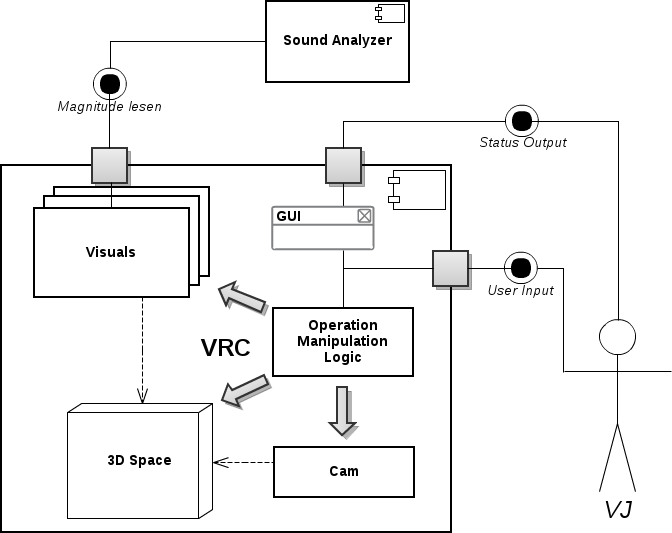
\includegraphics[width=1\textwidth]{pictures/vrc-component1.png}
    \caption{Strukturdarstellung des VJ-Konzeptprogramms VRC, bestehend aus Soundeingabe und einem Container f\"ur
    3D-Raum und Visuals welche von einem User f\"ur die VJ-Performance genutzt werden.}
\end{figure}

Das Konzept weist eine grundlegende Struktur aus 3D-Raum, Visuals, Soundeanalyse und Bedienkonzept auf


\subsection{\"Uberlegungen}

OpenGL entwickelte sich zum Industriestandard f\"ur interaktive 2D und 3D-Grafiken (* http://www.opengl.org/about/ )
und bietet eine umfangreiche Programmierschnittstelle f\"ur Grafikprogrammierung. Diese Schnittstelle wird durch
Grafikkarten hardwareseitig unterst\"utzt. F\"ur die meisten popul\"aren Sprachen gibt es Sprachanbindungen mit denen
man auf die Schnittstelle direkt zugreiffen kann. 

Spiel-Engines als Programmierger\"ust erscheinen vorteilhaft um 3D-Grafiken in Szene zu setzen. Durch die Beschr\"ankung
auf standard Eingabeget\"ate sind Spiel-Engines hervorragend f\"ur die Verarbeitung von Benutzereingabe und Steuerung
des 3D-Raums geeignet. Auch das Erstellen von Visuals erf\"ahrt durch die Verwendung von Spiel-Engines Vorteile. Elemente
werden in Visuals gruppiert und mit Funktionen unter Einbezug verschiedener Parameter modifiziert/transformiert. Anhand
des Soundsignals k\"onnen ausgew\"ahlte Parameter dem musikalischen Zufall \"uberlassen werden. Dadurch wird eine 
akustisch-visuelle Koppelung zwischen Visual und Umgebung m\"oglich. Die Soundeingabe soll m\"oglichst unabh\"angig von
technischen Faktoren m\"oglich sein. Laptops haben meist schon standardm\"a\ss{}ig ein Mikrofon eingebaut, das man als
standard Eingabeger\"at bei Performances nutzen kann. 

Wichtig vor allem ist, dass man Effekte durch Tastendruck ausl\"osen kann. Dazu m\"ussen Visuals frei programmierbar sein
um mit Code den Ablauf des Effekts zu definieren. Dadurch dass Tasten mit Programmierung belegt werden k\"onnen, sind f\"ur
die Visuals individuelle Funktionen programmierbar. Durch Anwendung der objektorientierten Programmierung k\"onnen 
Funktionen (Methoden) k\"onnen Objekte als Container f\"ur Funktionen und Daten dienen. Objektorientiertes Programmieren
eignet sich also f\"ur Visuals.


%OpenGL - Hardwarebeschleunigt
%Framework f\"ur OpenGL - Game Engine, SDL, Processing
%Mikrofon als Soundinput - standard laptops haben bereits mic
%Python/C++/Java - Comparision Libraries/Bindings
%Libraries - Soundanalyse, GUI, 
%Datenstrukturen f\"ur Visuals
%Visualrealisierung - OpenGL, eigene Funktionen

\subsubsection{Datenstrukturen}

Um die Visuals im Programm vorzuhalten und kann eine Liste mit Verweisen auf die Visuals verwendet werden. F\"ur 
die Visual-Elemente muss der 3D-Raum eine Datenstruktur vorhalten in den die Elemente hineingeladen werden k\"onnen.
Daf\"ur eignet sich eine Baumstruktur ganz gut. Der 3D-Raum stellt die Wurzel des Baums dar, jedes Visual ist ein
Kind des 3D-Raums. Ein Visual besteht aus einem Knoten, der als Wurzel f\"ur die Visual-Elemente fungiert
(siehe Abbildung). Dieser Baum stellt den Szenengraphen dar, in dem die OpenGL-Objekte der Visuals, wie Modelle, Texturen 
oder Videos geladen werden.

\begin{figure}[h!]
    \centering
    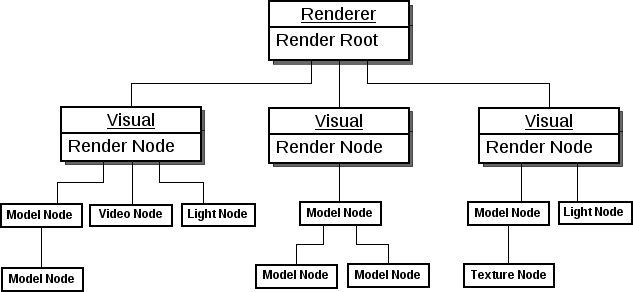
\includegraphics[width=1\textwidth]{pictures/data_structure1.png}
    \caption{Skizze eines Szenengraphen}
\end{figure}

%Liste mit VisualObjekt-Referenzen
%Visual-Elemente werden von Visuals in Graphen geladen
%VisualObjekt haelt Referenzen auf seine eigenen Elementobjekte im Graph der VisualElemente
%3D-Raum wird aufgebaut anhand des Graphen, der den zu sehenden Inhalt enth\"alt

\subsubsection{Soundanalyse}

Es gibt verschiedene M\"oglichkeiten Sound zu analysieren. Bei diesem Entwurf wird Wert darauf gelegt, dass 
Soundwerte auf einfache Art in den Visuals verarbeitet werden k\"onnen. Es sollen B\"asse, Mitten und H\"ohen
als Werte von  0 bis X abgelegt werden.

Die Soundanalysekomponente muss kontinuierlich die Soundeingabe verarbeiten. Das aufgenommene Frequenzband
wird unterteilt in Bassband, Mittelband und H\"ohenband. 
Das Bassband erstreckt sich \"uber die Frequenzen 0Hz bis 100Hz, die Mittelt\"one \"uber 100Hz bis 1000Hz,
und die Hoehen \"uber 1000Hz bis 44100Hz.
F\"ur jedes Band wird eine Magnitude berechnet, welche die Intensit\"at Samples auf den drei B\"andern angibt.
Dem Mikrofonsignal werden kontinuierlich Samples entnommen um die Magnitude \"uber den Frequenzb\"andern zu 
messen und in Soundzustandsvariablen zu speichern. Das Soundsignalsample ist ein Vektor aus 16Bit Integer-Werten -
f\"ur jede Frequenz ein Integer.

Eine einfache Methode den die Musik zu analysieren und einen Beat zu erkennen ist beispielsweise das Vergleichen
der Magnitude mit einem Grenzwert. Liegt die Magnitude \"uber dem Grenzwert, so kann das als Beat interpretiert
werden worauf eine Aktion folgen kann.

\subsubsection{Bedienung}

Da in den Anforderungen, die Benutzung von standard Eingabeger\"aten gefordert ist stellt vor allem die
Tastatur zur Steuerung von Visuals eine gute Plattform dar. Das Virtual Room Concept verh\"alt sich von der
Navigieren im 3D-Raum \"ahnlich dem des Bewegens von Aktoren in Computerspielen oder Arbeiten mit 3D-Programmen
wie Blender. In Computerspielen ist das was der Spieler sieht eine Ansicht einer virtuellen Kamera auf die ihn
virtuell umgebende Szenerie. Eine Grundlage zum Spielen ist das Bewegen des Agenten im Spiellevel, was dem 
Bewegen einer virtuellen Kamera in einem 3D-Raum entspricht.

Viele Spiele, allen voran First-Person-Spiele (FPS) haben oft f\"ur das Bewegen des virtuellen Agenten standardm\"a\ss{}ig
die selbe Tastenbelegung. Auch andere Funktionen wie die Auswahl von Gegenst\"anden ist oft \"ahnlich belegt.
Der gr\"o\ss{}te Unterschied zu den meisten FPS ist es wohl, dass man die Kamera, bzw die Visuals zus\"atzlich um die
L\"angsachse rotieren moechte.

In diesem Entwurf wird die Bedienung von FPS f\"ur die Kamera und Visuals adaptiert. F\"ur die Rotationen wird
auch die Tastatur verwendet. Hierf\"ur werden zus\"atzlich Belegungen definiert. Diese unterscheiden sich von
denen in FPS. In FPS wird f\"ur die den Nick- und Gier-Winkel h\"aufig die Maus verwendet. Da f\"ur Kamera und
Visual jeweils Rotationen und Bewegungen m\"oglich sein sollen, wird die Bedienung f\"ur diese Aktionen 
vereinfacht indem die selbe Belegung f\"ur Visual und Kamera gilt.

Die Abbildung zeigt den Entwurf f\"ur eine m\"ogliche Tastenbelegung.

\begin{figure}[h!]
    \centering
    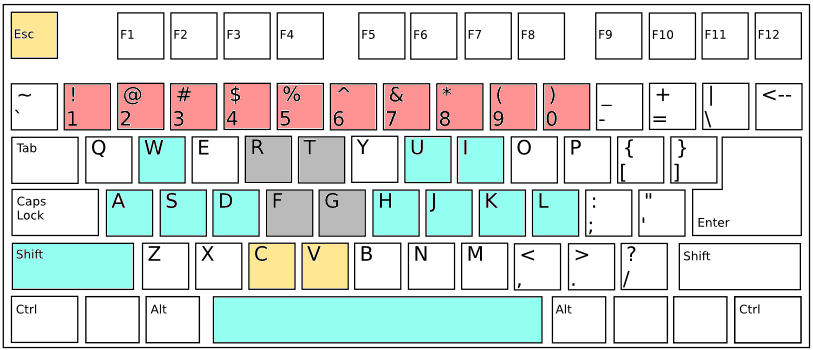
\includegraphics[width=1\textwidth]{pictures/usage_keyboard_layout1.png}
    \caption{Skizze eines Szenengraphen}
\end{figure}

F\"ur das Navigieren in der grafischen Oberfl\"ache wird die Maus verwendet.

%Tastatur, Maus
%Belegung Feste und programmierbare
%Bild

\subsubsection{Grafischen Oberfl\"ache}

In der grafischen Oberfl\"ache werden Daten aus dem Zustand des VRC aufbereitet, um Statusinformationen \"uber die
Visuals und Kamera anzuzeigen. Ausserdem werden \"uber die grafische Oberfl\"ache die Visuals in den 3D-Raum hinzugef\"ugt
oder entfernt. Wichtige gemeinsame Funktionen der Visuals k\"onnen in der grafische Oberfl\"ache zusammengefasst und 
der Manipulation zug\"anglich gemacht werden. 

Es m\"ussen die wichtigen Entit\"aten zum VJing schnell abrufbar sein. Gleichzeitig hat man aber nur begrenzten Platz auf
dem Bildschirm um Vorschaufenster und Menus unterzubringen.
Durch eine geschickte Unterbringung der Entit\"aten in Menus die mit Reitern navigierbar gestaltet sind, kann man Menuelemente
f\"ur den Visualpool, geladene Visuals, Kamera- und Soundeinstellungen gruppieren.
%Eine geschickte Unterbringung der Entit\"aten unter Reitern
%kann man seperat Visualpool, geladene Visuals, Kamera- und Soundeinstellungen erm\"oglicht das Gruppieren der verschiedenen
%Oberfl\"achenelemente. 
Die verschiedenen Entit\"aten Sound, Visuals und Kamera haben auch ihre eigenen Anforderungen an
Schnittstellen. So haben Visuals eine Schnittstelle f\"ur Skalierung, Transparenz, die Kamera aber nicht. Da es sich um
eine \"uberschaubare Menge an Entit\"aten handelt ist ein Reiterlayout f\"ur den VJ beim VJing ausreichend um Kontrolle
\"uber die Visualwerte zu behalten.

\begin{figure}[h!]
    \centering
    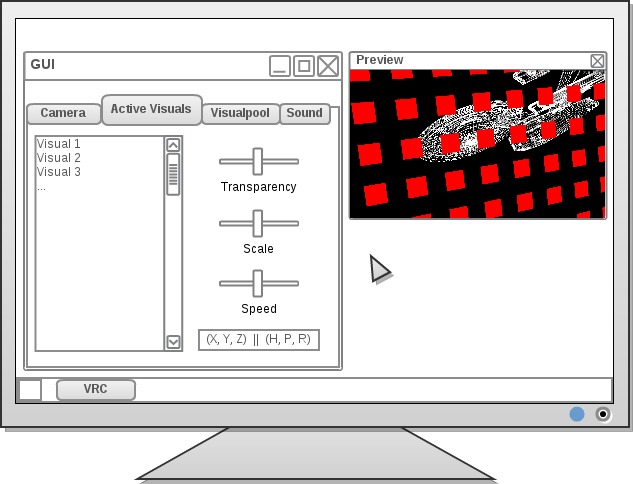
\includegraphics[width=1\textwidth]{pictures/gui1.png}
    \caption{Skizze der Grafischen Oberfl\"ache auf einem Monitor als Fenster f\"ur das Virtual Room Concept und die Vorschau}
\end{figure}

Das Resultat, welches auf im Vorschaufenster zu sehen ist wird auf \"uber einen zweiten Videoausgang ohne Fensterrahmen auf
einem externen Ausgabeger\"at angezeigt.


\subsubsection{Engine}

Letztendlich braucht man ein Framework, mit dem die Grafikausgabe programmiert werden kann. F\"r die verschiedenen anfallenden
Aufgaben braucht man einen Taskmanager, der wiederholende Aufgaben erledigt. Das Framework dient als Schicht zwischen OpenGL
und den zus\"atzlichen Komponenten wie Soundanalysierer und grafischer Oberfl\"ache.

Spiel-Engines besitzen Eigenschaften, die f\"ur sie Realisierung der Virtual-Room-Concept-Programms essentiell sind. Vor
allem bieten sie eine Datenstruktur zur Unterbringung der 3D-Geometrie - meist einen Szenengraphen in Baumstruktur.
Auf den Szenengraphen wird \"uber eine Schnittstelle in der Spiel-Engine zugegriffen. Ein Task-Manager der kontinuierlich
die Benutzereingaben und die Soundanalyse verwaltet erleichtert das Programmieren der Ablauflogik innerhalb des VRC-Programms.
Zum einen mussen die Visuals stets mit Soundwerten versorgt werden, zum Anderen m\"ussen die Eingaben des Benutzers
entgegengenommen und ausgef\"uhrt werden.

F\"ur die Visualprogrammierung ist die Wahl einer Spiele-Engine vorteilhaft, da man eine Abstraktionsebene f\"ur das 
Zusammenstellen von Geometrie und 3D-Modellen in den Szenengraphen hat. 
%Beim Performen der Visuals ist es wichtig die Visuals in die Szenerie laden und entfernen zu k\"onnen. 
Auch f\"ur das Performen eignen sich Spiele-Engines gut und besitzen dank des 
Szenengraphen und seinen Schnittstellen eine einfache M\"oglichkeit Visuals zu laden und zu entfernen. Die Betrachtung 
der Szenerie durch eine virtuelle Kamera ist eine grundlegende Anforderung f\"ur Spiel-Engines, sowie f\"ur das
VRC-Programm.

Das Angebot an freien Spiel-Engines ist relativ gro\ss{}, jedoch sollte die Spiel-Engine so gew\"ahlt werden, dass sie
sich gut mit den anderen  Komponenten des VRC-Programms und ihren Bibliotheken verwenden l\"asst. 

Neben vielen C++ und Java Spiel-Engines existieren auch f\"ur viele andere Sprachen Spiel-Engines. Dabei ist entscheidend,
dass die Spiel-Engine einen gro\ss{}en Benutzerkreis haben damit ein Interesse besteht, die Spiel-Engine auch in Zukunft
aktualisiert und weiterentwickelt werden.

Python erfreut sich in der 3D-Gestaltung einer hohen Popularit\"at. Programme wie Blender und auch Modul8 besitzen eine 
Python-Sprachanbindung. Blender verf\"ugt sogar \"uber eine eigene Spiel-Engine in Python. Mit Python als Sprache f\"ur 
eine Spiel-Engine erleichtert man durch die relativ einfache Syntax VJs den Einstieg in das Konzept. Eine gute Dokumentation
der Sprache und der Spiel-Engine hilft bei der Erstellung der Prototyps und der Visuals enorm. Anhand dieser Aspekte
l\"asst sich die Wahl einengen in eine OpenGL-basierte Spiel-Engine f\"r Python. Die bekanntesten Vertreter von 
Spiel-Engines f\"ur Python sind Python-Ogre, Spring, Blender oder Panda3d.

Weitere Vorteile von Spiel-Engines sind 
\begin{itemize}
    \item Konvertierungswerkzeuge f\"ur viele 3D-Modellingtools
    \item Shader-Generatoren f\"ur Spezialeffekte
    \item Kollisionsdetektion und Unterst\"utzung eines Physik-Systems
\end{itemize}

%Panda3d
%3d-Raum
%Kamera (eigene subsubsection)

%\subsubsection{Szenengraph}
%Renderer

\subsubsection{Visual-Klasse}

Visuals besitzen durch ihre Anforderungen an Beweglichkeit, Skalierung und andere gew\"unschte Manipulationsm\"oglichkeiten
eine Menge an gleichen Funktionen, welche diese Operationen umfassen. Da Visuals als Objekte gedacht sind l\"asst sich deren
Charakterisierung von einer Klasse ableiten.

\begin{wrapfigure}{r}{0.5\textwidth}
    \begin{center}
        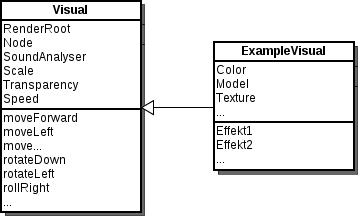
\includegraphics[width=0.48\textwidth]{pictures/visualclass1.png}
    \end{center}
    \caption{Visual-Klasse vererbt einem Visual-Objekt die n\"otigen Daten und Funktionen um im Programm an Soundanalyse
        und Szenengraph angebunden und einheitlich beweglich zu sein.}
\end{wrapfigure}

Durch die richtige Initialisierung und einer Standardeinstellung ist das \"Uberschreiben und Erweitern der Visual-Klasse im
Objekt m\"oglich.
Die Visual-Klasse besitzt einen Konstruktor mit dem die Initialisierung f\"ur das VRC-Programm vorgenommen wird. So wird
der Knoten, an den alle weiteren 3D-Elemente gekn\"upft werden erstellt, Referenzen auf andere Komponenten des
VRC-Programms werden angelegt.
Weiter werden Funktionen f\"ur die Bewegung und Rotation der Visuals schon in der Visual-Klasse definiert. Mit diesen 
Funktionenen ist es m\"oglich die Visuals im 3D-Raum anzuordnen.

Diese Eigenschaften k\"onnen von Visuals geerbt werden und stehen ihnen dann zur Verf\"ugung. Mit der Verwendung einer
Visual-Klasser erreicht man, dass sich Visuals trotz individueller Programmierung einheitlich in das VRC-Programm
einf\"ugen und steuern lassen.

\section{Prototyp}

\subsection{Softwarewahl}

Nach erfolglosen Versuchen mit Processing einen Prototypen zu erstellen begann die Suche nach Alternativen. Erst
wurden noch javabasierte Bibliotheken f\"ur OpenGL ausprobiert. Nachdem aber schnell klar wurde, dass keine der
getesteten Bibliotheken in der Lage war simpel und komfortabel zwei Fenster mit dem selben Inhalt darzustellen begann 
die fiel der Fokus auf Spiel-Engines. Wichtig wurde immer mehr, dass eine gute Dokumentation und eine gut aufgestellte 
freie Entwicklergemeinschaft wichtig sind f\"ur den Erfolg des Projekts. Durch eine gute Dokumentation ist es 
leichter die verwendete Software zu erlernen, dank einer aktiven Benutzer- und Entwicklergemeinschaft werden spezifische
Fragen in Internet-Foren oder Chat-R\"aumen schnell beantwortet.

Letzendlich fiel die Wahl der Game-Engine auf Panda3d. Mit Panda3d wurden zu Beginn Testprogramme erstellt, mit denen
die Anforderungen an Funktionalit\"at ausgetestet werden. So wurde erst einmal versucht die Ausgabe des Programms
auf einem undekorierten Fenster auf ein Ausgabeger\"at in Form von Videoprojektor auszugeben. Als diese Funktionalit\"at
durch kleine Testprogramme erreicht worden ist, ging es darum zu sehen, wie sich die Ansicht auf die 3D-Szenerie
bedienen l\"asst. Dazu wurde ein kleines Programm mit ein paar geladenen Models geschrieben und eine Kamera hineingesetzt.
Nachdem erfolgreich die Kamerabedienung programmiert worden ist, waren das die Kriterien f\"ur die Entscheidung bei der
verwendeten Spiel-Engine zu verbleiben und darauf aufzubauen. Wichtig bei der Wahl der Spiel-Engine war auch, dass 
sie nicht veraltet ist und Techniken wie Shaderprogrammierung, Schatten und Licht in verschiedenen Variationen besitzt und
eine klare Programmierkonvention hat. Panda3d erf\"ullt all diese Eigenschaften und noch viele Mehr wie Physik-Engine und
Shader-Unterst\"utzung.

F\"ur die Soundanalyse-Komponente ist wichtig, ohne gro\ss{}e Schwierigkeiten die Hardware anzusprechen und den Sound
dar\"uber auszulesen. Bei der Berechnung der Magnituden muss man \"uber ein Vektor aus 16Bit nat\"urliche Zahlen iterieren.
Dabei muss man die Laufzeit beachten. Es gibt Bibliotkeken f\"ur Python zum Auslesen des Signals \"uber Pulse-Code-Modulation.
Einen Algorithmus zur Berechnung der Magnitude auf den Frequenzb\"andern der tiefen, mittlere und hohen T\"one konnte
aus einem C++-Programm \"ubersetzt, welches eine \"anliche Soundanalyse-Komponente verwendete (reference auf liveGL von phreax)

Panda3d bietet die M\"oglichkeit verschiedene Wrapper f\"ur GUI-Toolkits zu verwenden, darunter wxPython (ref)  und TKinter (ref).
WxPython ist ein Wrapper f\"ur die wxWidgets-Klassenbibliothek (ref), TKinter ist eine Sprachanbindung an den Tk (ref). 
Tkinter entwickelte sich zum quasi-standard GUI-Paket f\"ur Python und wird mit Python zusammen ausgeliefert.
Tkinter eignet sich zum schnellen Prototypenbau f\"ur grafische Oberfl\"achen. F\"ur den VRC-Prototypen wurde die
Tkinter-Bibliothek gew\"ahlt.

\subsection{Datenstrukturen}

Innerhalb der Testprogramme wurden Datenstrukturen f\"ur die Bedienung und das Handhaben der Visuals verwendet.
Dabei erwies sich assoziatives Datenfeld als geeignet, um die Tastatureingabe entgegenzunehmen und f\"ur ein 
Bedienschl\"usselwort zu speichern. Panda3d verarbeitet Tastendruck- und Tastenfreigabe-Events. Die Tastenzust\"ande
lassen sich bin\"ar als 1 und 0 darstellen, wobei 1 gedr\"uckt repr\"asentiert und 0 nicht gedr\"uckt bedeutet.
Um nun f\"ur eine Operation den Zustand zu speichern wird die Tastatur zyklisch abgefragt. Wenn eine Taste gedr\"uckt wird
und einer Operation entspricht so wird der Wert dieser Operation auf 1 gesetzt, wie anhand des Codebeispiels gezeigt.

\begin{lstlisting}

if key == "a": setOperationMap('move-forward', 1)
if key == "a-up": setOperationMap('move-forward', 0)

\end{lstlisting}

So wird der Zustand der Eingabe an einer Stelle im Speicher vorgehalten und ist in anderen Teilen des
Prototypen leicht abrufbar.

In einer Listen werden die Verweise auf geladene Visuals vorgehalten. Dadurch k\"onnen Funktionen leicht auf allen
geladenen Visual-Objekten ausgef\"uhrt werden, wie beispielsweise das Versorgen mit den Sound-Messwerten.

Der Szenengraph ist eine baumartige Datenstruktur. Panda3d besitzt Schnittstellen um Knoten und deren Unterknoten
aus dem Baum zu entfernen und an einer anderen Stelle im Szenengraphen anzuh\"angen. So k\"onnen Visuals, die nicht mehr
performt werden sollen aus dem Graph entfernt werden wodurch Rechenressourcen frei werden.

\subsection{Software-Architektur}

Das Zusammenf\"uhren von Visuals, Sound-Messwerten und GUI erfordert eine durchdachte Architektur f\"ur das VRC-Programm.
Die erforderlichen Komponenten lassen sich zu Klassen zusammenfassen. Das Klassendiagramm (siehe Abb X) zeigt die 
Assoziationen der Klassenobjekte untereinander.

\begin{figure}[h!]
    \centering
    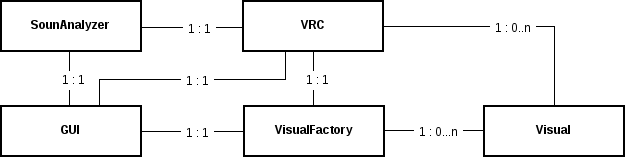
\includegraphics[width=1\textwidth]{pictures/classdiagram1.png}
    \caption{grobes Klassendiagramm mit Assoziationen}
\end{figure}

\subsubsection{VRC-Klasse}

Die VRC-Klasse erbt von der Spiel-Engine. So bekommt sie unter Anderem die Puffer f\"ur den 3D-Raum und den Taskmanager 
vererbt, die die Grundlage f\"ur das Konzept bilden. Mithilfe des Taskmanagers kann man wiederkehrende Tasks wie 
das Abfragen des SoundAnalyzers und des Tastaturzustands ausf\"uhren. Dadurch vermeidet man das Programmieren in einer 
Hauptschleife.
In ihrem Konstruktor initialisiert die VRC-Klasse, die f\"ur sich ben\"otigten Objekte der anderen Klassen.
In Variablen und einer Liste f\"ur Visuals werden die Referenzen auf diese Objekte gespeichert.

Neben den f\"ur das Konzept wichtigen Objekte, wird in der VRC-Klasse auch die Initialisierung der Spiel-Engine
vorgenommen. Unter anderem werden Fenster erstellt, und die Kameras den Fenstern zugewiesen.

\begin{figure}
\begin{lstlisting}
props = WindowProperties()
props.setSize(size)
props.setUndecorated(True)
props.setOrigin(0,0)
self.otherWin = self.openWindow(props, makeCamera = 0)
self.win.setClearColor((0,0,0,1))
self.otherWin.setClearColor((0,0,0,1))
\end{lstlisting}
\end{figure}

Ausserdem wird in der VRC-Klasse der Bedienmechanismus implementiert. Der Bedienmechanismus schaltet zwischen
Visualmodus und Kameramodus zwischen Funktionen um, die f\"ur die Tastatureingabe in dem assoziativen Datenfeld
f\"ur Operationen richtig schalten. Daf\"ur wird mithilfe des Taskmanagers der Spiel-Engine der Tastaturzustand
kontinuierlich abgefragt und anhand dessen die Aktionen ausgef\"uhrt.
Die Spiel-Engine implementiert anhand von Event-Polling das Belegen
von Tasten mit Funktionen. 
Da die VRC-Klasse von der Spiel-Engine erbt kann man ganz Einfach im Konstruktor die Belegung
der n\"otigen Tasten initialisieren und an Funktionen kn\"upfen.

\begin{lstlisting}
self.accept('a', self.setOperation, ['a'])
self.accept('a-up', self.setOperation, ['a-up'])
...
self.taskMgr.add(self.executeOperation, 'keyboardaction')
self.taskMgr.add(self.spreadTheBeat, 'sound')
\end{lstlisting}

In der executeOperation-Funktion wird anhand des Bedienmodus die entschieden ob die Kamera-Operationen oder
Visual-Operationen ausgef\"uhrt werden. Die spreadTheBeat-Funktion f\"uhrt auf allen Visuals eine Methode zum
Reagieren auf. Dadurch erhalten die Visuals gleichzeitig einen Art Tick, anhand Sie selbst kontinuierlich 
Funktionen implementieren k\"onnen.

\subsubsection{SoundAnalyzer-Klasse}

In der Soundanalyzer-Klasse werden Bibliotheken f\"ur die Schnelle Fouriertransformation und f\"ur den Zugriff
auf das PCM-Signal verwendet um \"uber die drei Frequenzb\"ander B\"asse, Mittelt\"one und H\"ohen das Spektrum
zu analysieren und als Gleitkommazahl zu repr\"asentieren.



\subsubsection{Visual-Klasse}

Die Visual-Klasse stellt Methoden f\"ur das Bewegen und Rotieren der Visuals bereit. Sie wird mit einer Referenen
auf den SoundAnalyzer und auf den 3D-Raum initialisiert.
Es wird ein Platzhalter-Knoten f\"ur den Szenengraph angelegt, der Ausgangspfad f\"ur die anderen Elemente des Visuals ist.
Dieser Knoten wird in den Bewegungsmethoden verwendet um das Visual durch den Raum bewegen zu k\"onnen. Alle Elemente,
die an diesen Knoten angef\"ugt werden bewegen sich dann relativ zum Platzhalter-Knoten mit.

\begin{lstlisting}
def __init__(self, render, loader, snd):
    self.snd = snd
    self.loader = loader
    self.render = render
    self.path = self.render.attachNewNode('dummy')
    self.path.setPos(0,0,0)
    ...
    self.setup()

def moveRight(self):
    self.path.setX(self.path, +self.visualMovementSpeed)
\end{lstlisting}

Au\ss{}erdem werden noch initiale Zustandsvariablen f\"ur die Bewegungsgeschwindigkeit, Transparenz und Skalierung definiert.
Der Konstruktor ruft zum Abschluss noch eine weitere leere Setup-Funktion auf. Diese Funktion ist daf\"ur gedacht,
als Framework-Funktion in den von der Visual-Klasse abgeleiteten Visuals \"uberschrieben zu werden. Dadurch kann man
an diesem Punkt die visualspezifischen Elemente laden und einstellen.

Weiter wird eine Methode f\"ur das Entgegennehmen der Soundanalyse implementiert. Diese Methode ruft noch eine weitere
Platzhalter-Methode auf, die im eigentlichen Visual dann mit einem Algorithmus f\"ur das Reagieren auf den Sound
\"uberschrieben werden kann.

F\"ur die Effekte werden leere Methoden angelegt, die aus der VRC-Klasse durch die Bedienung ausgel\"ost werden. In den
einzelnen Visuals k\"onnen diese Methoden \"uberschrieben werden. Dadurch hat man ein Framework um sich f\"ur die
Tasten eigene Effekte anlegen zu k\"onnen.

\subsubsection{VisualFactory-Klasse}

Der Prototyp verwendet f\"ur das Initialisieren der Visuals eine Visual-Objektfabrik, da die Initialisierung eines Visuals
mehr als da Initialisieren des Konstruktor ben\"otigen kann. Dadurch hat man als Programmierer mehr Freiheiten aus dem
Visual-Framework auszubrechen und Ideen zu Realisieren, welche die Anbindung anderer Externer Bibliotheken oder Module
erfordern.
Der Konstruktor nimmt Referenzen auf 3D-Raum und SoundAnalyse-Objekt entgegen um damit die Visuals zu initialisieren.
Die Visual-Objekte werden unter einem Namen in einem W\"orterbuch angelegt.

\subsubsection{GUI}

In der GUI befinden sich Slider, Buttons und Listen mit denen die Einstellungen an Kamera, Visuals und SoundAnalyzer 
vorgenommen werden k\"onnen. So wird \"uber die GUI mithilfe von Schiebern die Transparenz, 
die Bewegungsgeschwindigkeit und Skalierung f\"ur die Visuals eingestellt. Mit einem Button k\"onnen die Visuals in den
Raum gesetzt und entfernt werden. Standardm\"a\ss{}ig werden die Visuals am Nullpunkt gesetzt. Die Namen der geladenen
Visuals erscheinen in einer Auswahlliste. Dort kann man ein Visual ausw\"ahlen, um es zu im Visualmodus bedienen.
F\"ur die Kamera kann die Sensitivit\"at \"uber einen Schieber eingestellt werden. Zur Soundanalyse koennen anhand von
drei Schiebern ein Grenzwert eingestellt werden, mit dem dann in den Visuals der aktuelle Messwert verglichen werden kann.
Dadurch kann man z.B. bei basslastigem Klang den Grenzwert erh\"ohen um die Reaktion der Visuals auf starke B\"asse zu 
trimmen. 

F\"ur den \"Uberblick sind Labels vorgesehen in denen die Positions- und Rotationsinformationen der Kamera und der Visuals
anzeigen. Au\ss{}erdem werden Informationen aus der dem Operationsw\"orterbuch angezeigt, wie bspw. ob die Kamera
im Vorschaufenster synchron mit der Kamera im Pr\"asentationsfenster ist, oder ob die Kamera auf ein Visual fixiert oder
frei ist.

\section{Usability Test}

Die Gebrauchstauglichkeit und Benutzbarkeit wird qualitativ anhand von vier Testpersonen ermittelt. Die Personen sollen
sich mit dem Programm vertraut machen, und die Bedienung ausprobieren. Danach wir den Testpersonen das VJing-Konzept
erkl\"art. Den Testpersonen werden Herangehensweisen f\"ur das Einfaden und Ausfaden der Visuals 
gezeigt, um das Potential des Konzepts vorzustellen. 

Nachdem die ersten Fragen der Testperson gekl\"art sind wird Musik abgespielt und das Programm neu gestartet. Die Testperson
muss von vorne starten ein Szenerie aufzubauen und eine Betrachtungsweise daf\"ur zu finden. Mittels Effekten und Transparenzen
wird versucht f\"ur ein bisschen visuelle Abwechslung zu Wendepunkten in der Musik zu sorgen.

Nachdem sich die Testperson mit \"Ubergangsmethoden und Effekten vertraut gemacht hat, und gelernt hat sich im 3D-Raum zu
orientieren, Visuals zu Positionieren und die Kamerabewegungen beherrscht, wird ein Szenario gestellt. Die Testperson soll 
sich vorstellen auf einem Konzert zu drei Liedern Visuals performen. Dazu wird Hiphop und Elektronische Tanzmusik 
verwendet. Bei Hiphop gibt es oft beim Refrain eine musikalische \"Anderung. Beispielsweise setzt ein zus\"atzliches 
Instrument ein oder es wird in einer Pause kurz innegehalten und der Beat setzt wieder ein. Bei elektronischer 
Tanzmusik sind Mittelt\"one, B\"asse und H\"ohen meistens gut voneinander unterscheidbar. Oft werden mit Tief- und
Hochpassfiltren gearbeitet um sogenannten Druck aufzubauen. Dabei wird die Musik mit Tiefpassfiltern ged\"ampft und wieder
aufgedreht. In solchen Momenten kann man irgend eine Aktion mit einem Visual oder mit der Kamera durchf\"uhren.

W\"ahrend des Test wurden die \"Au\ss{}erungen der Testpersonen in Stichw\"ortern notiert. Da die Testpersonen 
unterschiedlichen Hintergrund haben, bringen sie unterschiedliche F\"ahigkeiten mit. Es testeten ein Fussballer ohne viel
Computerkenntnisse, eine Linguistikstudentin, die Programmiergrundlagen beherrscht,
ein Filmemacher der Dozent f\"ur neue Medien und Film an der Universit\"at Siegen ist und ein Student
mit einer Leidenschaft f\"ur Computerspiele. 

Die Aussagen der Testperson werden im Folgenden anhand der Notizen zusammengefasst und einer Evaluation unterzogen. 
Die Ergebnisse sollen Kriterien f\"ur den zweiten Prototypen werden.

\subsection{Testperson 1: Benutzer mit wenig Computerkenntnissen}

Die erste Testperson hat in ihrem Alltag gar nichts mit Computern zu tun. Privat verwendet die Person den Computer nur um
Sportergebnisse nachzuschauen und Musik im Internet zu h\"oren. Die Testperson war dementsprechend offen f\"ur ein Konzept,
das keine Gemeinsamkeiten mit den Erfahrungen der Testperson hat. 

Spielerisch probierte die Person die Tastatureingaben aus.
Die Bedienung konnte schnell erlernt werden. Jedoch hatte die Person Schwierigkeiten eine Performance zu gestalten und
\"Uberg\"ange oder Effekte in den richtigen Momenten vorzunehmen.

Zur Tastenbelegung der Bedienung machte die Person keine Angaben. Bei der Benutzung der grafischen Oberfl\"ache fand die
Person es aber irritierend, dass das zuletzt angeklickte Visual nicht automatisch das aktive Visuals ist.

F\"ur Szenenkomposition w\"unschte sich die Person eine Speicherfunktion, so dass man Szeneneinstellungen abspeichern kann.
Dabei soll die Position, Rotation, Kameraposition und Blickwinkel gespeichert werden k\"onnen.

Die Testperson hatte zudem Schwierigkeiten mit der Orientierung im 3D-Raum, da es keine Orientierungspunkte gibt und 
schlug Reset-Funktion vor, mit der man die Kamera wieder auf Aufgangslage bringen kann.

\subsection{Testperson 2: Benutzer mit grundlegenden Programmierkenntnissen}

Die zweite Testperson verf\"ugte \"uber grundlegende Programmierkenntnisse und war au\ss{}erdem bereit auch Visuals zu 
erstellen.

Bei der Benutzung fand die Tastaturbedienung f\"ur Neigung, Rotation und Drehung unlogisch und fand die Bedienung 
nicht intuitiv. Trotzdem sagte die Testperson, die Bedienung sei schnell erlernbar. Die Benutzung allgemein wurde 
als un\"ubersichtlich kritisiert, da die Person nicht schnell auffassen konnte in welchem Modus sie sich befand.

Auch diese Person hatte Probleme sich in dem Raum zu orientieren. F\"ur das Erlernen der Funktionen wie Soundanalyse
hielt die Person kleine Erkl\"arungsk\"asten f\"ur hilfreich. Als Orientierungshilfe schlug sie eine Gitterstruktur auf
der XY-Ebene vor.

Zur Performance kritisierte die Person einen zu komplizierten Ablauf. Da man ein Fenster hat, in dem die Spiel-Engine
l\"auft und ein Fenster f\"ur die grafische Oberfl\"ache muss man zwischen den Fenstern wechseln, damit die Tastatureingabe
wieder in der Spiel-Engine funktioniert, wenn man davor etwas in der grafischen Oberfl\"ache verstellt hat.

Auch diese Person fand, dass eine Abspeicherfunktion von Positionierung und Performance hilfreich w\"are.

Beim erstellen von Visuals fand die Person das Framework ersichtlich und sinnvoll gestaltet. Zusammen wurde ein Visual
erstellt.

\subsection{Testperson 3: Benutzer mit Erfahrung im Medienbereich}

Die dritte Testperson hat Erfahrung mit Videobearbeitungsprogrammen, unter anderem AfterEffects von Adobe, mit dem man
unter anderem 3D-Animationen erstellen kann. Dabei arbeitet man auch mit einer virtuellen Kamera in einem 3D-Raum. 
Dadurch hatte die Testperson keine Schwierigkeiten mit dem Betrachtungskonzept und arbeitete vor allem damit.
Au\ss{}erdem hat die Testperson schon einmal als VJ auf einer Party eine Performance mit Resolume und Videoclips realisiert.

Interessanter Weise fand diese Person das Bedienkonzept ganz gut. Mit der Orientierung hatte sie keine Probleme und
benutzte die Kamerafunktionen ausgiebig. Schlie\ss{}lich fand sie sich auch mit den Kamera-Toggle-Kn\"opfen zurecht und 
konnte Schnitte erstellen.

Bei der Performance passten die von mir pr\"aparierten Visuals aber nicht. Die Testperson w\"unschte sich vor allem andere
Visuals. Auch fand diese Testperson viele Labels in der GUI unn\"otig und die Umschaltung der Bedienmodi ein bisschen 
aufw\"andig, meinte aber dass man sich daran gew\"ohnen kann. Die Idee alles per Tastaturk\"urzel zu regeln wurde
angesprochen und die GUI nur auf das wichtigste zu reduzieren. Vor allem die verschiedenen Tabs zum Umschalten wurden 
kritisiert. Die Zusammenf\"uhrung aller wichtigen Regler auf einer gemeinsamen Fl\"ache w\"are sinnvoll. So w\"urden 
die Bedienwege verk\"urzt. Die wichtigsten Labels der Koordinaten k\"onnte man auch platzsparend in einer Zeile plazieren
k\"onnen.

Zwar konnte der Person das Erstellen von einem Visual erkl\"art werden, aber aufgrund keiner Kenntnisse im Programmieren
wurde nur dar\"uber diskutiert. Jedoch aus eigener VJ-Erfahrung gefiel der Person das Konzept des getesten Prototyps.

\subsection{Testperson 4: Computerspieler}

Die vierte Testperson hatte aufgrund ihrer Erfahrungen mit verschiedenen Computerspielen viele Verbesserungsvorschl\"age
bez\"uglich der Bedienung. Die Bedienung wurde als schlecht bewertet. Das wechseln der Bedienmodi wurde kritisiert. Anstatt
die ESC-Taste zum Verlassen des aktuellen Modus zu dr\"ucken, k\"onnte man auch direkt in den gew\"unschten Modus wechseln.

Trotz Allem unterbreitete die Person viele Verbesserungsvorschl\"age. Die Testperson bemerkte die Toggle-Tasten f\"ur die
Kamera und argumentierte, dass man genauso gut mit Toggle-Tasten auf Visual-Einstellungen wie Transparenz, Skalierung 
und Geschwindigkeit f\"ur das Inkrementieren und Dekrementieren der Werte benutzen k\"onnte. So w\"urde man eine
Toggle-Taste dr\"ucken und anschlie\ss{}end mit zum Beispiel den Pfeiltasten den Wert ver\"andern. Dadurch w\"urde 
die grafische Oberfl\"ache nur noch zur Orientierung und Statusanzeige existieren. 


Die Testperson schlug au\ss{}erdem vor mit der Maus per Klick in das Vorschaufenster mit der Mausbewegung die Rotation
der Szenerie zu erm\"oglichen w\"ahrend man die Maustaste gedr\"uckt h\"alt. 
An der Kamera wurde eine zu hohe Rotationssensitivit\"at kritisiert.

%Dabei wurden manche Dinge von
%jeder Testperson bemerkt, jedoch unterschiedlich stark vertieft. Vor allem f\"ur die Bedienung hatten alle Testpersonen 
%verschiedene Beobachtungen und Vorschl\"age. Alle Testpersonen haben das Programm nach etwa einer halben Stunde erlernen
%k\"onnen, trotzdem war die Bedienung f\"ur keine Person intuitiv. 

\subsection{Evaluation}

Der erste Prototyp gen\"ugte den Anforderungen an Benutzbarkeit offensichtlich noch nicht ganz. Man kann zwar schon alle
Funktionen bedienen, jedoch stiftet die Trennung zwischen Spiel-Engine und grafischer Oberfl\"ache Verwrirrung.
Bei dem Testversuch waren sich alle Personen einig, dass die Bedienung hinsichtlich der Zugriffschnelligkeit verbessert werden 
muss. W\"ahrend Einstellungen in der grafischen Oberfl\"ache vorgenommen worden sind und daraufhin eine weitere Aktion 
in der Spiel-Engine stattfinden soll, indem man mit per Tastatur weiterperformt, gerieten die Testpersonen in Schwierigkeiten.
Das Wechseln der Fenster beeintr\"achtigte das auf den richtigen Moment abgestimmte Performen. H\"aufig passierte
im Spiel-Engine-Fenster dann auch nichts, da die Testperson sich noch in keinem Bedienmodus befand.

Sobald eine Szenerie angeordnet worden war und die Testpersonen damit ihre Idee performen konnten, w\"unschten sie sich
eine Abspeicherfunktion. Die Abspeicherfunktion wurde mit dem vorhergehenden Aufwand begr\"undet eine passende Szenerie
nicht jedes mal neu erstellen zu m\"ussen.

F\"ur die Verbesserung des Prototyps konnte die vierte Testperson gute Ideen beitragen.




\section{Verbesserter Prototyp}

\section{Zweiter Test}

\section{Resultat}
